\documentclass[]{article}
\usepackage{mathrsfs}
\usepackage{amsmath}
\usepackage{amsfonts}
\usepackage{graphicx}
\usepackage[left=20mm, right=20mm, top=20mm, bottom=20mm]{geometry}


\begin{document}
\huge Transformada de Laplace.
\\

\normalsize Para comenzar a entender la transformada de Laplace debemos tener en claro como funciona la transformada de Fourier. Recordemos la definición.
\\
La transformada de Fourier de una función $f(t)$ se define:
$$
F(\omega) = \int_{-\infty}^{\infty}f(t)e^{-i\omega t} dt 
$$
\\
La transformada de Fourier venía acompañada de una condición necesaria que decía que $f(t)$ debe ser seccionalmente continua y de módulo integrable en todo el eje real, por ello muchas funciones no eran transformables ya que el area encerrada bajo la curva de estás tendería a infinito cuando $t\rightarrow \infty$.

Para solucionar esto, es conveniente multiplicar por un factor exponencial decreciente $e^{-\alpha t }$ obteniendose:
$$
\int_{-\infty}^{\infty} f(t) \cdot  e^{-\alpha t}\cdot  e^{-i\omega t}dt =
\int_{-\infty}^{\infty} f(t) \cdot  e^{-st}
$$
con $s=\alpha + i \hspace{3pt} \omega $
\\ Y esta es la definición de la transformada de Laplace. Esta, al igual que la transformada de Fourier se aplica en el dominio del tiempo, pero nos devuelve una funcion en un dominio de vairable compleja $s$ que llamaremos dominio de Laplace.
\\ Dentro del enfoque de la materia se trabajará con la versión unilateral de la transformada bajo la supocisión que todas las funciones $f(t)$ trabajadas cumpliran 
$f(t) = 0  \hspace{10pt} \forall t < 0$.
$$
F(s) = \int_{0}^{\infty} f(t) e^{-st} dt
$$

\large Teorema de existencia.
\\

\normalsize Sea $f(t)$ una función seccionalmente continua y $f(t)$ de orden exponencial $\gamma$ para $t > N \Rightarrow \exists \hspace{5pt} \mathscr{L}[f(t)]$

Una función $f(t)$ es de orden exponencial $\gamma \Longleftrightarrow$ ${\exists \hspace{5pt} M,\gamma \in \mathbb{R}  / \forall t > N: |e^{-\gamma t} f(t)| < M }$ si $t \rightarrow \infty$.

Es decir, la función en módulo no puede crecer mas que $Me^{\gamma t}$ a partir de un cierto valor $N$.


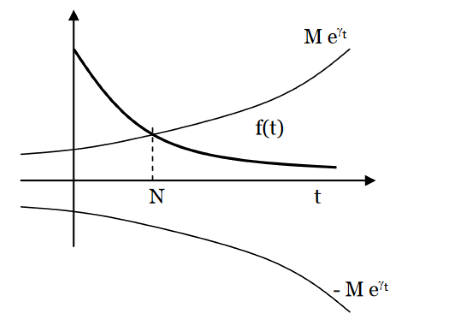
\includegraphics{../../../Imagenes/Superior/Superior01.PNG}

\large Propiedades de la transformada de Laplace
\normalsize
\\
\\
$a)$ Linealidad
$$
F(s) = \mathscr{L}[f(t)]\hspace{7pt} \wedge\hspace{7pt} G(s) = \mathscr{L}[g(t)]\hspace{7pt} \wedge\hspace{7pt} k_{1} , k_{2} \in \mathbb{R} \Rightarrow \mathscr{L}[k_{1}f(t) + k_{2}g(t)] = k_{1} F(s) + k_{2} G(s)
$$
\\
\\
$b)$ Primera propiedad de traslación

$$
F(s) = \mathscr{L}[f(t)] \Rightarrow \mathscr{L}[e^{at}f(t)] = F(s-a)
$$
Esto significa que multiplicar por $e^{at}$ en el dominio del tiempo, equivale a efectuar una traslación de $a$ unidades hacia la derecha en el dominio de Laplace.
\\
\\
$c)$ Segunda propiedad de traslación

$$
F(s) = \mathscr{L}[f(t)] \hspace{5pt} \wedge \hspace{5pt} g(t) = \left\{
	\begin{array}{ll}
		f(t-a) \hspace{10pt} t > a \\
		0 \hspace{40pt} t < a
	\end{array}
\right. \\
\Rightarrow \mathscr{L}[g(t)] = e^{-as}F(s)
$$

Esto significa que una traslación de $a$ unidades hacia la derecha en el dominio del tiempo equivale a multiplicar por $e^{-as}$ en el dominio de Laplace.
\\
\\
$d)$ Cambio de escala


$$
F(s) = \mathscr{L}[f(t)] \Rightarrow \mathscr{L}[f(at)] = \frac{1}{a}F(\frac{s}{a})	
$$
\\
\\
$e)$ Transformada de las derivadas

$$
F(s) = \mathscr{L}[f(t)] \Rightarrow \mathscr{L}[f^{n}(t)] = s^{n}\cdot F(s) -s^{n-1}f(0) - s^{n-2} f'(0) - \dots - f^{n-1}(0)
$$
Se puede encontrar una relación entre esta propiedad y el binomio de Newton. Al avanzar en la sumatoria (de restas) el grado de $s^{n}$ va decreciendo mientras que el "grado" (orden) de la derivada de $f(0)$ va aumentando.\\
Además vale la pena observar que una derivada en el dominio del tiempo, se traduce a un polinomio en el dominio de Laplace, esto junto con la propiedad siguiente será muy util para resolver ecuaciones diferenciales e integrodiferenciales.
\\
\\
$f)$ Transformada de la integral simple

$$
F(s) = \mathscr{L}[f(t)] \Rightarrow \mathscr{L}[\int_{0}^{t}f(u)du] = \frac{F(s)}{s}
$$
\\
\\
$g)$ Multiplicación por $t^{n}$

$$
F(s) = \mathscr{L}[f(t)] \Rightarrow \mathscr{L}[t^{n}f(t)] = (-1)^{n}F^{(n)}(s)
$$
Es decir, multiplicar por $t^{n}$	en el dominio del tiempo equivale a derivar en el orden $n$ en el dominio de Laplace.
\\
\\
$h)$ División por t

$$
F(s) = \mathscr{L}[f(t)] \Rightarrow \mathscr{L}[\frac{f(t)}{t}] = \int_{s}^{\infty}F(u)du
$$
Esto es valido siempre que $\exists \lim_{t\rightarrow 0} \frac{f(t)}{t}$
Es decir, dividir por $t$ en el dominio del tiempo, equivale a integrar en el dominio de Laplace. Observar que en el dominio de Laplace tenemos una función integral, al resolver nos quedará una función de $s$ como cualquier otra transformada.
\\
\\
$i)$ Teorema del valor inicial

Si existen los limites indicados, se cumple:

$$
\lim_{t\rightarrow 0} f(t) = \lim_{s\rightarrow \infty} sF(s)
$$
\\
\\
$j)$ Teorema del valor final

$$
\lim_{t\rightarrow \infty} f(t) = \lim_{s\rightarrow 0} sF(s)
$$

Observar que en estas ultimas dos propiedades la transformada está multiplicada por $s$
\\
\\
$k)$ Transformada de funciones periódicas
4
$$
f(t) = f(t+T) \Rightarrow F(s) = \mathscr{L}[f(t)] = \frac{1}{1-e^{-sT}}\int_{0}^{T}e^{-st}f(t)dt
$$
\\
\\

\large Funciones utiles
\normalsize
\\

Estas son algunas funciones muy elementales y nos serán utiles para calcular transformadas de Laplace sin tener que usar la definición. Nos basaremos en estas funciones y haremos todos los calculos teniendo en cuenta las propiedades detalladas anteriormente.

\Large
$$
\setlength{\tabcolsep}{20pt}
\renewcommand{\arraystretch}{1.5}
\begin{tabular}{|c|c|}
	\hline
	\textbf{$f(t)$} & \textbf{$\mathscr{L}[f(t)] = F(s)$}\\
	\hline
	
	$1$ & $\frac{1}{s}$ \\

	\hline
	$t$ & $\frac{1}{s^{2}}$ \\
	\hline
	$t^{n}$ & $\frac{n!}{s^{n+1}}$ \\
	\hline
	$e^{at}$ & $\frac{1}{s-a}$ \\
	\hline
	$\sin{at}$ & $\frac{a}{s^{2}+a^{2}}$ \\
	\hline
	$\cos{at}$ & $\frac{s}{s^{2}+a^{2}}$ \\
	\hline
	$\delta(t)$ & $1$ \\
	\hline
\end{tabular}
$$

\normalsize
La función $\delta(t)$ es una funcíon especial y será explicada mas adelante.
\\
\\
\large Funciones especiales.
\normalsize
\\

Son funciones muy utilizadas dentro de la ingenieria y nos permiten modelar ciertos sistemas comunes. Además nos facilitaran el calculo de ciertas transformadas.
\\
\\
\large Función escalón unitario

\normalsize


$$
E(t) = \left\{
	\begin{array}{ll}
		1 \hspace{10pt} t > 0 \\
		0 \hspace{10pt} t < 0
	\end{array}
\right. \\
$$
o bien
$$
E(t-a) = \left\{
	\begin{array}{ll}
		1 \hspace{10pt} t > 0 \\
		0 \hspace{10pt} t < a
	\end{array}
\right. \\
$$
\\
Esta función es muy importante, ya que multiplicada por una constante ,puede representar funciones constantes apartir de un cierto instante $a$. Es muy util para representar una señal de tensión continua, o una fuerza constante aplicada sobre algún sistema mecánico.

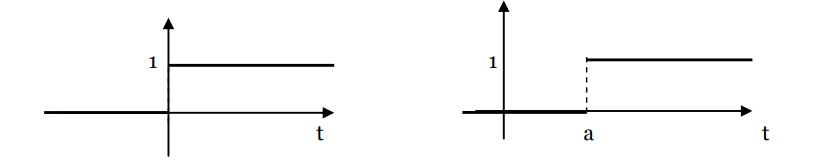
\includegraphics{../../../Imagenes/Superior/Superior02.PNG}

La trasnformada de $E(t)$ aparece en la tabla y la de $E(t-a)$ es muy sencilla de calcular con la segunda propiedad de traslación.
$$
\mathscr{L}[E(t)] = \frac{1}{s}
$$
$$
\mathscr{L}[E(t-a)] = \frac{e^{-as}}{s}
$$

Además la función $E(t-a)$ resulta muy util para considerar funciones a partir de un cierto instante y definir funciones por trozos.
Consideremos el siguiente ejemplo:

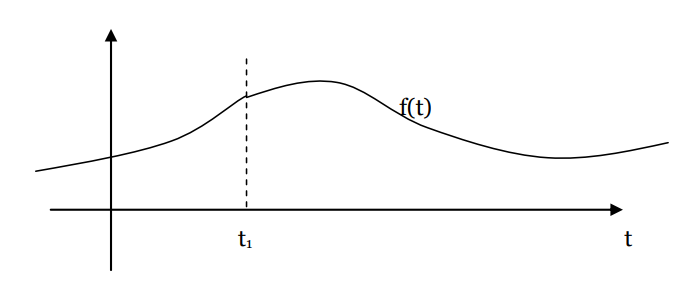
\includegraphics{../../../Imagenes/Superior/Superior03.PNG}


Si multiplicamos $f(t)$ por $E(t-t_{1})$ obtenemos: 

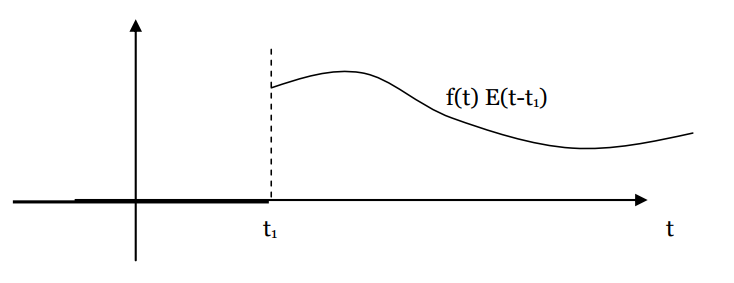
\includegraphics{../../../Imagenes/Superior/Superior04.PNG}

Como $E(t-t_{1})$ vale $0$ antes de $t_{1}$ al multiplicar por $f(t)$ esta se reduce a $0$, y despues de $t_{1}$ la funcion $f(t)$ queda igual porque se está multiplicando por $1$.

Veamos ahora un ejemplo aún mas util que nos facilitará el calculo de una transformada. Como ya mencionamos, la funcíon $E(t)$ nos ayuda a la hora de escribir funciones por partes y ciertamente nos ayudará a calcular su transformada.

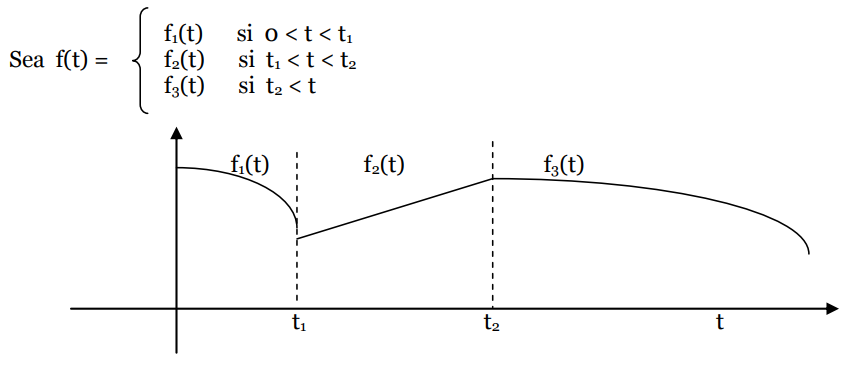
\includegraphics{../../../Imagenes/Superior/Superior05.PNG}


Entonces $f(t)$ puede ser escrita de la siguiente forma.
$$
f(t) = f_{1}(t)\cdot (E(t)-E(t-t_{1})) + f_{2}(t) \cdot (E(t-t_{1})-E(t-t_{2})) + f_{3}(t)E(t-t_{2})
$$
Simplificaremos la notación para resolver los calculos mas facil llamando:
\begin{align}
E(t) &= E_{0} \\
E(t-t_{1}) &= E_{t_1} 
\end{align}
Entonces se deduce:
\begin{align}
  f(t) &= f_{1}(t)\cdot (E_0-E_{t_1}) + f_{2}(t) \cdot (E_{t_1}-E_{t_2}) + f_{3}(t)E_{t_2} \\
f(t) &= f_1(t)E_{0} - f_1(t)E_{t_{1}} + f_2(t)E_{t_{1}} - f_2(t)E_{t_2} +f_3(t)E_{t_2} \\
f(t) & = f_1(t)E_0 + E_{t_1}\cdot(f_2(t) - f_1(t)) + E_{t_2}\cdot(f_3(t)-f_2(t))
\end{align}
Al aplicar la transformada queda:
\begin{align}
  F(s) &= \mathscr{L}[f_1(t)E_0 + E_{t_1}\cdot(f_2(t) - f_1(t)) + E_{t_2}\cdot(f_3(t)-f_2(t))] \\
  F(s) &= \mathscr{L}[f_1(t)E_0] + \mathscr{L}[E_{t_1}\cdot(f_2(t) - f_1(t))] + \mathscr{L}[ E_{t_2}\cdot(f_3(t)-f_2(t))] \\
  F(s)& = \mathscr{L}[f_1(t)] + e^{-t_1s}\cdot (\mathscr{L}[f_2(t)] - \mathscr{L}[f_1(t)]) + e^{-t_2s} \cdot(\mathscr{L}[f_3(t)]-\mathscr{L}[f_2(t)]) 
\end{align}
\\
\\
\large Función impulso unitario
\\
\normalsize



\end{document}